\chapter{Multiclausal constructions}
\label{chapter10-2}
\setcounter{enums}{0}

\noindent As discussed previously, one of the main motivations for
using \isi{ICONS} (Individual CONstraints)\is{Individual CONStraints}
is to capture binary relations across clauses.\is{binary relation}
This chapter looks into how the relations between matrix clauses and
non-matrix clauses are represented via ICONS. Since \isi{ICONS} is a
way of representing a relation between an individual and a clause that
the individual belongs to, it is necessary to identify the relation
between two clauses in a single sentence.  This chapter also looks at
the restrictions non-matrix clauses have with respect to information
structure.  Many previous studies argue that information structure in
non-matrix clauses is differently formed from that in matrix clauses.
For example, according to \citet{kuno:73}, \wa in \ili{Japanese} is
seldom used in relative clauses.\is{relative clause} Similarly,
(\ref{exe:rizzi:306}a) indicates that \ili{English} normally disallows
\isi{left dislocation} in relative clauses.

\myexe{\eenumsentence{\label{exe:rizzi:306}
\item{*A man who your book\mysub{i} could buy it\mysub{i}.}
\item
{Un uomo che, il tuo libro\mysub{i}, lo\mysub{i} potrebbe comprare. \\
A man who, your book, could buy it. [ita] \citep[306]{rizzi:97}}}}

\noindent However, this restriction is language-specific.  Embedded
clauses in some languages exhibit properties of root clauses as shown
in (\ref{exe:rizzi:306}b).  Furthermore, \citet{haegeman:04} argues
that \isi{topic} \isi{fronting} can occur in non-root clauses even in
\ili{English} under certain circumstances, such as adversative clauses,
\textit{because} clauses, and sometimes conditional clauses.  This
restriction is related to so-called embedded root phenomena
\citep{heycock:07}.\is{root phenomena}
While a root clause is most simply defined as a
clause that is not embedded, there exist some counterexamples to such
a definition. It is known that root phenomena have an effect on the
appearance of topics in embedded clauses. For instance,
\citet{portner:yabushita:98} insist that topic should only be
interpretable with the wide scope on the root clause.  OSV word order
constructions in English and \wa-marking in \ili{Japanese} typically
exhibit a root effect in that they tend not to appear in non-root
clauses.



Non-matrix clauses can be roughly classified into at least three
types.  These are complement clauses
(Section \ref{10:ssec:embedded}),\is{complement clause} relative clauses
(Section \ref{10:ssec:relative}),\is{relative clause} and adverbial clauses
(Section \ref{10:ssec:adjunct}).\is{adverbial clause} Each section in this
chapter looks into linguistic factors that have an influence on
information structure in each clausal type,\is{HPSG}\is{MRS} and
provides an HPSG/MRS-based analysis of the clausal type.




\section{Complement clauses}
\label{10:ssec:embedded}


The issues that this section addresses include how components of
information structure are constituted in complement
clauses,\is{complement clause} and how assignment of information
structure values is conditioned in different complement clauses.
Dependency graphs in \myref{fig:complement:clauses} show the basic
mechanism of indexing between TARGETs and CLAUSEs in multiclausal
constructions.\is{CLAUSE}\is{TARGET} In accordance with the AVMs
presented hitherto, (\ref{fig:complement:clauses}a--c) are the
representations of a sentence \textit{Kim thinks that the dog
  barks}. In (\ref{fig:complement:clauses}a), the subject in the
matrix clause is B-accented, and the subject in the embedded clause is
A-accented.\is{A-accent}\is{B-accent} Hence, they are assigned
\tdl{contrast-or-topic} and \tdl{semantic-focus},\is{semantic focus}
respectively \mypage{avm:fc:tp:eng}. The arc from the main verb
\textit{thinks} to the verb in the embedded clause \textit{barks}
comes from the lexical information of the main verb, which inherits
from \tdl{one-icons-lex-item}. That is, \textit{thinks} has one
inherent element on its ICONS list, which links its own INDEX to INDEX
of \textit{barks}.\footnote{These underspecified \tdl{info-str}
  elements are not fully desirable.\is{\textit{info-str}} An analysis
  that allows specific \isi{ICONS} elements relating the two clauses
  but does not entail inserting these underspecified ones is left for
  future work.\is{underspecification}}





\myexe{\enumsentence{\label{fig:complement:clauses}
\begin{tabular}[t]{ll}
a. & \evnup{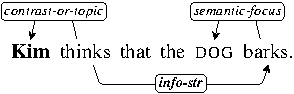
\includegraphics{pdf/embedded1.pdf}}\\
b. & \evnup{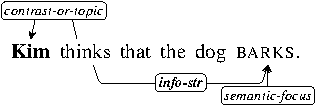
\includegraphics{pdf/embedded2.pdf}} \\ 
c. & \evnup{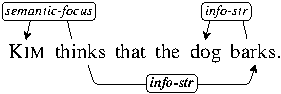
\includegraphics{pdf/embedded3.pdf}} \\
\end{tabular}}}




\subsection{Background}
\label{10:ssec:embedded:background}




Topic can sometimes occur in complement clauses,\is{complement clause}
largely depending on the characteristics of the predicate in the main
clause.  The properties that license topics to appear in complement
clauses include speech acts, semi-factives, and quasi-evidentials
\citep{roberts:11}.  \citet{maki:etal:99} argue that \isi{topic}
\isi{fronting} in embedded clauses in \ili{English} and appearance of \wa in
embedded clauses in \ili{Japanese} commonly exhibit four
characteristics as given in \myref{def:maki}.\footnote{In the previous
  studies, topic-marking (also known as topicalization) and meaning of topic
  seem to be used without distinction. Nonetheless, we can say that
  topic can be marked even in embedded clauses and the topic-marked
  constituents can be potentially interpreted as conveying topic
  meaning.}



\myexe{\eenumsentence{\label{def:maki}
\item{Embedded topicalization is possible in complement clauses of
  bridge verbs (e.g.\ \textit{believe}, \textit{sinziteiru}
  `believe').}
\item{Embedded topicalization is possible in interrogative
  clauses.}
\item{Embedded topicalization is impossible in complement clauses of
  factive verbs (e.g.\ \textit{regret}, \textit{kookaisiteiru}
  `regret') and noun-complement clauses.\is{complement clause}}
\item{Embedded topicalization is impossible in an adjunct clause
  and in a sentential subject. \citep[8--10]{maki:etal:99}}}}

\noindent \citet{heycock:07}, in a similar vein, elaborates on cases
in which embedded clauses have a root function.  According to
\citeauthor{heycock:07}'s analysis, the main criterion to distinguish
whether sentential subjects/complements exhibit root phenomena or not
is assertion. In other words, whether a \isi{topic} can occur in subordinate
clauses is influenced by whether the subordinate clause is asserted.
A five-way division of predicates is offered as follows.\is{root phenomena}


\myexe{\eenumsentence{\label{def:heycock}
\item Class A predicates (e.g.\ ``say'', ``report'', ``be true'', ``be
  obvious''). The verbs in this group are all verbs of saying. Both
  the verbs and the adjectives in this group can function
  parenthetically, in which case the subordinate clause constitutes
  the main assertion of the sentence. It is claimed however that if
  the subordinate clause occurs in subject position (as in,
  e.g.\ ``\textit{That German beer is better than American beer is
    true}'') it is not asserted.
\item Class B predicates (e.g.\ ``suppose'', ``expect'', ``it seems'',
  ``it appears''). In this group also the predicates can function
  parenthetically, and in this case the subordinate clause is
  asserted. The distinction between this group and Group A is not made
  entirely clear, although it is noted that Class B predicates allow
  ``Neg raising'' and tag questions based on the subordinate clause.
\item Class C predicates (e.g.\ ``be (un)likely'', ``be
  (im)possible'', ``doubt'', ``deny'') have complements which are not
  asserted.
\item Class D predicates (e.g.\ ``resent'', ``regret'', ``be odd'',
  ``be strange''); these factive predicates have complements which are
  argued to be presupposed, and hence not asserted.
\item Class E predicates (e.g.\ ``realize'', ``know''); these
  semifactives (factives that lose their factivity in questions and
  conditionals) have a reading on which the subordinate clause is
  asserted. \citep[189]{heycock:07}}}



\noindent Based on the division presented in
\myref{def:heycock},\is{complement clause} complement clauses may or
may not contain a topicalized phrase, depending upon whether the
predicate of the matrix clause belongs to Class A, B, or E.


Moreover, \isi{contrastive topic} can relatively freely appear in embedded
clauses.  \citet{bianchi:frascarelli:10} examine embedded
topicalization in \ili{English}.\is{complement clause} In short, their
conclusion is that a contrastive topic (C-Topics in their terminology)
interpretation is readily available within complement clauses. In
other words, although the complement clauses are not endowed with
assertive force, an interpretation of contrastive topic is acceptable
by native speakers.  This claim shows a similarity to the analysis of
\onun-marked phrases in \ili{Korean} relative clauses
(Section \ref{3:sssec:clausal-constraints}).\is{relative clause} If \nun
appears in relative clauses as presented below, the \onun-marked
constituent is evaluated as containing a contrastive meaning
\citep{lim:12}.\is{contrast}

\myexe{\enumsentence{\label{exe:lim:14:ch10-2}
\shortex{4}
  {hyangki-nun & coh-un & kkoch-i & phi-n-ta.}
  {scent-\textsc{nun} & good-\textsc{rel} & flower-\textsc{nom} & bloom-\textsc{pres}-\textsc{decl}}
  {`A flower with a good scent blooms.' [kor] \citep[229]{lim:12}}}}




\subsection{Analysis}
\label{10:ssec:embedded:analysis}

Two restrictions are factored into constraining information
structure in complement clauses.\is{complement clause}

First, \isi{topic} fronting can happen even in embedded clauses. Some
languages, such as \ili{Italian}, do not impose any restriction on
topic \isi{fronting} in embedded clauses \citep{roberts:11}. Even in
languages which have such a restriction (e.g.\ \ili{English},
\ili{Japanese}, and \ili{Korean}), constituents can be topicalized in
embedded clauses if the constituents carry a contrastive meaning as
shown in \myref{exe:lim:14:ch10-2}.  The topicalized constituents in
complement clauses would have to be evaluated as containing
\tdl{contrast-topic} in my intuition.  At least in English,
\ili{Japanese}, and \ili{Korean}, the clear-cut distinction between
contrastive topics and non-contrastive topics does not matter in
generating sentences,\is{contrastive topic}\is{non-contrastive topic}
because the meaning difference between them is
not marked in surface forms.  One potential problem can be found in
languages which employ different marking systems for contrastive
topics and non-contrastive topics. Recall that Vietnamese uses
\textit{th{\`i}} for expressing contrastive topics but not for marking
non-contrastive \isi{topic} \citep{nguyen:06}.\footnote{Topic-marking
  systems in embedded clauses in Vietnamese-like languages need to be
  further examined in future work.}


Second, if the main verb is one of the members of verbs of saying
(\textit{say}), semi-factive verbs (\textit{realize}), and
quasi-evidential verbs (\textit{it appears}), the complement clause
can be asserted,\is{complement clause} and thereby the structural
relation between main and complement clauses is normally (but not
always) specified as \tdl{focus}.\is{focus}  Otherwise, the complement clause
has an underspecified relation (i.e.\ \tdl{info-str}) to its matrix
clause(s).\is{underspecification}



For instance, since the main verb \textit{appears} in
\myref{fig:it-appears} is quasi-evidential, it has an arrow to
\textit{read} in complement clauses, whose value is specified as
\tdl{focus}. Note that the syntactic subject \textit{it} is an
expletive (i.e.\ semantically and informatively vacuous), and does not
have any information structure relation to the clause.\footnote{There
  could be some counterexamples to this analysis. Further work will
  examine the full range of information structure relations that
  complement clauses have to their main clauses.}

\myexe{\enumsentence{\label{fig:it-appears}
\evnup{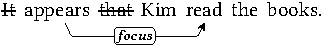
\includegraphics{pdf/it-appears.pdf}}}}

\noindent \textit{Appears} in \myref{fig:it-appears}, accordingly, has
the following structure.

\myexe{\enumsentence{\label{avm:appears}
\evnup{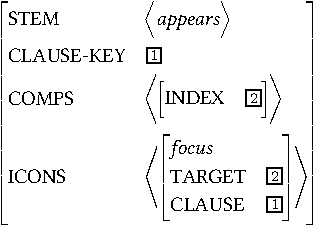
\includegraphics{pdf/appears.pdf}}}}


\section{Relative clauses}
\label{10:ssec:relative}

Which information structure value is assigned to the head noun
modified by relative clauses?\is{relative clause} The behaviors of
information structure shown by relative clauses have been analyzed
from three points of view in previous literature: (i) Relative clauses
assign \isi{topic} to their modificands or the relative pronouns
\citep{kuno:76,bresnan:mchombo:87,jiang:91,bjerre:11}.  (ii) Relative
clauses do not always give a topic meaning to the head NPs
\citep{ning:93,huang:etal:09}.  (iii) Relative clauses signal \isi{focus} on
the head nouns \citep{schachter:73,schafer:etal:96}. This subsection
examines each perspective, and offers a new approach to the
information structure properties that relative clauses have in
relation to their relativized constituents.\footnote{A deeper details
  of analyzing information structure of relative clauses 
  is provided in \citet{song:14b}.}


\subsection{Background}
\label{10:ssec:relative:background}



First, \citet{bresnan:mchombo:87} and \citet{bjerre:11} claim that
relative pronouns indicate a \isi{topic} function, as stated
before.\is{relative pronoun} For convenience sake, the analysis that
\citeauthor{bresnan:mchombo:87} provide is shown again below.

\myexe{\enumsentence{\label{exe:bresnan:mchombo:87:eng:rel}
\begin{tabular}[t]{l}
\evnup{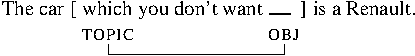
\includegraphics{pdf/bresnan-mchombo-eng-rel.pdf}} \\
\mbox{ } \mbox{ } \mbox{ } \mbox{ }
\mbox{ } \mbox{ } \mbox{ } \mbox{ }
\mbox{ } \mbox{ } \mbox{ } \mbox{ }
\mbox{ } \mbox{ } \mbox{ } \mbox{ }
\mbox{ } \mbox{ } \mbox{ } \mbox{ } 
\mbox{ } \mbox{ } \mbox{ } \mbox{ } 
\mbox{ } \mbox{ } \mbox{ } \mbox{ }\citep[757]{bresnan:mchombo:87}
\end{tabular}}}



\noindent \citet{bjerre:11} provides a similar analysis to
\myref{exe:bresnan:mchombo:87:eng:rel}. This analysis is presented in
an example \myref{exe:anne:rel} in \ili{Danish}.
\citeauthor{bjerre:11},\is{clefting} making use of clefting as a tool
to diagnose \isi{focus}, claims that (\ref{exe:anne:rel}b),\is{clefting}
which has a clefted relative pronoun \textit{den}, is of dubious
acceptability.  Whereas (\ref{exe:anne:rel}a), in which an
interrogative pronoun \textit{hvem} is clefted, sounds normal. Recall
that focus and \isi{topic} are mutually exclusive in the present study.


\myexe{\enumsentence{\toplabel{exe:anne:rel}
\evnup{\begin{tabular}[h]{lllllllllll}
a. &Som & komponist \xspace & er & det & naturligvis \xspace & vigtigt,  \\
   &as & composer & is & it & of course & important \xspace \\ 
\end{tabular}}
\newline
\evnup{\begin{tabular}[h]{lllllllllllll}
\hphantom{a.}   & at & lytterne & ved, \\
   & that & listeners.\textsc{def} \xspace & know \\
\end{tabular}}
\newline
\evnup{\begin{tabular}[h]{lllllllllllll}
\hphantom{a.}   & \myemp{hvem} & det & er & der & har & skrevet & den \xspace musik, \\
   & \myemp{who} & it & is & there \xspace & has & written & that \xspace music\\
\end{tabular}}
\newline
\evnup{\begin{tabular}[h]{lllllllllllll}
\hphantom{a.} & de & lytter & til. \\
 & they & listen & to \\
\end{tabular}}
\newline
\evnup{\begin{tabular}[h]{lllllllllllll}
   & \multicolumn{11}{l}{`As a composer it is of course important that the listeners know}\\
   & \multicolumn{11}{l}{who it is that has written the music they are listening to.'}\\
\end{tabular}}
\newline
\evnup{\begin{tabular}[h]{lllllllllllll}
b. & ???Som \xspace & komponist & er & det & naturligvis & vigtigt, \\
   & as & composer & is & it & of course & important \\
\end{tabular}}
\newline
\evnup{\begin{tabular}[h]{lllllllllllll}
\hphantom{b.}    & at & lytterne & kender \\
   &  that & listeners.\textsc{def} \xspace & know \\
\end{tabular}}
\newline
\evnup{\begin{tabular}[h]{lllllllllllll}
\hphantom{b.}   & \myemp{den} & musik & hvilken \xspace & det & er & der & lyttes & til. \\
   & \myemp{that} & music & which & it & is & there & listen.\textsc{prs}.\textsc{pas} \xspace & to \\
   & \multicolumn{11}{l}{`As a composer it is of course important that the listeners know}\\
   & \multicolumn{11}{l}{that music which it is that is listened to.' [dan] \citep[279]{bjerre:11}}
\end{tabular}}}}


However, attempts to apply their approach to the current work are
blocked by three key issues.\is{relative pronoun} Two of them are
related to distributional properties of relative pronouns, and the
other is related to system-internal factors.  The first and the most
important problem is that relative pronouns do not necessarily exist
in all human languages. \ili{Japanese} and \ili{Korean}, for example,
do not have relative pronouns, and relative clauses in these languages
are constructed in a different way \citep{baldwin:98,kim:park:00}. If
relative pronouns were universally to be evaluated as bearing the
\isi{topic} function, all relative clauses in Korean and Japanese
would be topicless constructions.\is{topicless} A second issue is that
relative pronouns can be missing in some circumstances even in
\ili{English} (e.g.\ those corresponding to object nouns in
restrictive readings). Since English is not a topic dropping language
(e.g.\ Chinese, Japanese, Korean, etc.), the dropped relative pronouns
would therefore be rather difficult to explain with respect to
information structure.\is{relative pronoun} Lastly, as hypothesized in
Section \ref{9:sec:hypotheses}, relative pronouns are syncategorematic and
their lexical type inherits from \tdl{no-icons-lex-items} which has an
empty list of ICONS. Hence, relative pronouns within the current work
cannot participate in building up the list of ICONS, though they can
perform a role in signaling information structure values on their
heads and/or dependents.





The first two problems posed above may be (partially) resolved by the
following constraint \citep[19f]{bresnan:mchombo:87}.\is{relative
  pronoun} That is to say, when there is no relative pronoun,
relativized constituents would play the same role.

\myexe{\enumsentence{\label{def:kuno}
The thematic constraint on relative clauses: A relative clause
  must be a statement about its head noun. \citep[420]{kuno:76}}}


\noindent \citeauthor{kuno:76} provides several examples in
\ili{Japanese} and \ili{English} to verify \myref{def:kuno}. First of all,
\citeauthor{kuno:76} argues (\ref{exe:kuno:jpn:rel}a) is derived from
not (\ref{exe:kuno:jpn:rel}b) but (\ref{exe:kuno:jpn:rel}c), in which
\textit{sono hon} `the book' occurs sentence-initially with the \isi{topic}
marker \wa to signal the theme (i.e.\ topic in the present study).
Recall that the constituent associated with aboutness topic usually
shows up in the initial position in Japanese
\citep{maki:etal:99,vermeulen:09}.\is{aboutness topic}


\myexe{\eenumsentence{\toplabel{exe:kuno:jpn:rel}
\item\shortex{4}
{[Hanko-ga & yonda] & hon}
{Hanako-\textsc{nom} & read & book}
{`The book that Hanako read'}
\item\shortexnt{5}
{[Hanko-ga & sono & hon-o & yonda] & hon}
{Hanako-\textsc{nom} & the & book-\textsc{acc} & read & book}
\item\shortexnt{5}
{[[sono & hon-wa]$_{\textnormal{{\tiny theme}}}$ & Hanko-ga &  yonda] & hon}
{the & book-\textsc{wa} & Hanako-\textsc{nom} & read & book [jpn] \citep[419]{kuno:76}}}}


At first glance, the explanation about the linguistic phenomena
presented above sounds reasonable.  It seems clear that relative
clauses present certain constraints on information structure. Yet, it
is still necessary to verify whether the head nouns modified by
relative clauses always and cross-linguistically carry the meaning of
\isi{topic}. Several previous studies present counterarguments to
\myref{def:kuno}.



\citet{huang:etal:09},\is{relative clause} from a movement-based
standpoint, basically accepts that topics and relative clauses share
some characteristics with \textit{wh}-constructions as
A$^\ensuremath{\prime}$-movement structures. The common properties
notwithstanding, they argue that relative clause structures are not
derived from topic structures for two reasons, contra \citet{kuno:76}.
First, a \isi{topic} relation does not license a relative construction in
Chinese.  For instance, if a topic structure were sufficient for
relativization in Chinese, (\ref{exe:hunag:etal:rel}b) and its
relativized counterpart (\ref{exe:hunag:etal:rel}c) would be equally
acceptable.


\myexe{\eenumsentence{\toplabel{exe:hunag:etal:rel}
\item\shortex{2}
{yiwai & fasheng-le}
{accident & happen-\textsc{le}}
{`An accident happened.'}
\item\shortex{3}
{tamen, & yiwai & fasheng-le}
{they & accident & happen-\textsc{le}}
{`(As for) them, an accident happened.'}
\item\shortex{5}
{*[[yiwai & fasheng-le & de] & neixie & ren]}
{accident & happen-\textsc{le} & \\textsc{de} & those & person}
{`the people such that an accident happened' [cmn] \citep[212--213]{huang:etal:09}}}}


\noindent In other words, \citeauthor{kuno:76}'s claim
\myref{def:kuno} is not cross-linguistically true.  Second,
\citet{ning:93} reveals that a relativized construction may be
well-formed even though its corresponding \isi{topic} structure is
ill-formed.  Thus, the well-formedness of a topic structure is neither
necessary nor sufficient for the acceptability of a corresponding
relative structure at least in Mandarin \ili{Chinese}.\is{relative
  clause}


\citet{schachter:73} probes into the relationship between \isi{focus}
constructions (e.g.\ clefts)\is{clefting} and restrictive relative
constructions, and concludes that they bear a striking likeness to
each other. On the basis of the findings from four languages including
\ili{English}, \ili{Akan}, \ili{Hausa}, and \ili{Ilonggo} (an
Austronesian language spoken in the Philippines),
\citeauthor{schachter:73} sets up a hypothesis: both constructions
syntactically necessitate the promotion of a linguistic item from an
embedded clause into the main clause, and semantically involve
foregrounding (i.e.\ making a specific part of a sentence conspicuous
at the expense of the rest). The following examples in Akan [aka] and
Ilonggo [hil] show that constructions involving relative clauses and
\isi{focus} constructions are structurally quite similar to each other.



\myexe{\eenumsentence{\toplabel{exe:aka:hil}
\item\shortex{4}
{\`{a}b\`{o}f\`{r}\'{a} & \'{a}\`{a} & m\'{i}h\'{u}\`{u} & n\'{o}}
{child & that & I.saw & him}
{`a child that I saw'}
\item\shortex{4}
{\`{a}b\`{o}f\`{r}\'{a} & n\`{a} & m\'{i}h\'{u}\`{u} & n\'{o}}
{child & that & I.saw & him}
{`It's a child that I saw.' [aka] \citep[108]{croft:02}}
\item\shortex{6}
{babayi & nga & nag- & dala & sang & bata}
{woman & that & \textsc{ag.top}- & bring & \textsc{nontop} & child}
{`the woman that brought a child'}
\item\shortex{7}
{ang & babayi & and & nag- & dala & sang & bata}
{\textsc{top} & woman & \textsc{top} & \textsc{ag.top}- & bring & \textsc{nontop} & child}
{`It was the woman who brought a child' [hil] \citep[108]{croft:02}}}}


\noindent One difference between (\ref{exe:aka:hil}a) and
(\ref{exe:aka:hil}b) is which marker (i.e.\ a relative marker \vs a
\isi{focus} marker) is used.\is{relative marker} As exemplified earlier in
Section \ref{4:sec:lexical}, \textit{n\`{a}} in (\ref{exe:aka:hil}b) behaves
as a focus marker in \ili{Akan}, and is in complementary distribution
with a relative marker \textit{\'{a}\`{a}} in
(\ref{exe:aka:hil}a). The same goes for (\ref{exe:aka:hil}c) and
(\ref{exe:aka:hil}d) in \ili{Ilonggo}.\is{relative clause} The
relative marker \textit{nga} and the second \isi{topic} marker \textit{ang}
share the same position to draw a boundary between the promoted NP and
the relative clause or the cleft clause.




The structural similarity notwithstanding,\is{relative clause} we
cannot conclude from the given examples that the head nouns of
relative clauses always bear the \isi{focus} function. We cannot even say
that a structural likeness is equal to likeness of information
structure meaning.\is{clefting} There are certainly formal
similarities between cleft constructions and relative clauses, but
these do not necessarily imply a corresponding similarity in
information structure meanings.



\subsection{Analysis}
\label{10:ssec:relative:analysis}

In sum, there are opposing arguments about the information structure
properties assigned to the head nouns of relative clauses. Thus, it is
my understanding that it is still an open question whether relative
clauses assign their head nouns a \isi{focus} meaning or a \isi{topic}
meaning. Moreover, previous studies show that the relation could
ultimately be language-specific.\is{relative clause} The present study
does not rush to create a generalization and instead allows a flexible
representation: The information structure values of the constituents
modified by relative clauses should be \tdl{focus-or-topic}, which is
the supertype of both \tdl{focus} and \tdl{topic} within the hierarchy
of \tdl{info-str} (Figure~\ref{fig:info-str}). This means that the
relativized constituents can be evaluated as delivering either focus
in some cases or topic. In the present framework then, information
structure in constructions involving relative clauses is analyzed
analogously to focus/topic \isi{fronting} constructions
(Section \ref{10:sec:fronting}). The preposed constituents in focus/topic
fronting constructions carry ambiguous meanings but for the help of
contextual information, and because of this they have to be flexibly
specified as \tdl{focus-or-topic}. The same motivation goes for
relativized constituents.



The present analysis also highlights the difference between
restrictive readings and non-restrictive readings of relative clauses
with respect to the \tdl{info-str} values they assign.\is{relative
  clause}


First, restrictive relative clauses and non-restrictive relative
clauses have been regarded as having different linguistic behaviors in
most previous work.  To begin with, there is an orthographic
convention in \ili{English} of setting off non-restrictive relatives with
commas, and not using commas for ordinary restrictive
relatives.\footnote{The use of comma is just
a convention in writing style, rather than a mandatory requirement for
a non-restrictive reading. That is, even though the comma does not
appear before (and after) a relative clause, we cannot say that the
relative is necessarily restrictive until the contextual information
is clearly given. In the present study, commas are inserted just for ease of
  comparison.} Syntactically, it has been stated that the distinction
between restrictive readings \vs non-restrictive ones yields different
bracketing as presented in \myref{exe:rel:brackets}.\is{relative
  clause} The restrictive relative clause in (\ref{exe:rel:brackets}a)
modifies the head noun \textit{dog} itself, and then the entire NP
\textit{dog which Kim chases} is combined with the determiner as
\tdl{head-spec-phrase}.  In contrast, the non-restrictive relative
clause in (\ref{exe:rel:brackets}b) modifies the NP in which the noun
\textit{dog} takes the determiner beforehand.  They also show
contrastive syntactic behavior in binding of anaphora
\citep{emonds:79}, co-occurrence with NPIs (e.g.\ \textit{any}), and
focus sensitive items (e.g.\ \textit{only}) \citep{fabb:90}.\is{focus
  sensitive item}\is{contrast}




\myexe{\eenumsentence{\toplabel{exe:rel:brackets}
\item{[[The [dog that Kim chases]] barks.]}
\item{[[[The dog,] which Kim chases,] barks.]}}}


\noindent Semantically, they may not share the same truth-conditions.\is{truth-conditions}


\myexe{\eenumsentence{\toplabel{exe:rel:truth}
\item Kim has two children that study linguistics.
\item Kim has two children, who study linguistics.}}


\noindent (\ref{exe:rel:truth}b) implies that Kim has two and only two
children, while (\ref{exe:rel:truth}a) does not. For example, if Kim
has three children, the proposition of (\ref{exe:rel:truth}b) would
not be felicitously used, whereas that of (\ref{exe:rel:truth}a) may
or may not be true depending on how many children among them study
linguistics.  Given that restrictive and non-restrictive relative
clauses exhibit different properties in semantics as well as syntax,
it is a natural assumption that they behave differently with respect
to information structure as well.



Beyond the general properties that restrictive relative clauses and
non-re\-stric\-tive relative clauses have, there is a distributional
reason for viewing them differently with regard to their information
structure.

\myexe{\eenumsentence{\toplabel{exe:rel:para}
\item Kim chases the dog that likes Lee. 
\item Kim chases the dog, which likes Lee. 
\item Kim chases the dog, and it likes Lee. 
\item Kim chases the dog, and as for the dog, it likes Lee.
\item Kim chases the dog, and speaking of the dog, it likes Lee.}}

\largerpage[-1]
\noindent Unlike restrictive relative constructions such as
(\ref{exe:rel:para}a),\is{relative clause} non-re\-stric\-tive
constructions such as (\ref{exe:rel:para}b) can be paraphrased into
(\ref{exe:rel:para}c--e). (\ref{exe:rel:para}c) reveals that
non-re\-stric\-tive relatives are almost equivalent to coordinated clauses
which clearly involve root phenomena
\citep[177]{heycock:07}.\is{root phenomena} In
(\ref{exe:rel:para}c), a pronoun \textit{it} is used as referring to
\textit{the dog} in the previous clause, which means \textit{the dog}
cannot receive \tdl{focus} from the non-restrictive clause in
(\ref{exe:rel:para}b). The focused constituents in the non-restrictive
clause should be either the object \textit{Lee} or the VP
\textit{likes Lee}.  Finally, the relative clauses in
(\ref{exe:rel:para}d--e) conclusively pass the test for aboutness
topic.\is{focus}\is{topic}\is{aboutness topic}














In sum, the semantic head of relative clauses (i.e.\ the verb in
relative clauses) basically has a \tdl{focus-or-topic} relation with
relativized dependents.\is{relative clause} Non-re\-stric\-tive relatives
additionally have a more specific constraint;
\tdl{aboutness-topic}.\is{aboutness topic} The schema of those constraints is exemplified
in the following dependency diagrams. The information structure
relations between \textit{dog} and the verb in the main clause
\textit{barks} are underspecified in these diagrams, because for now
there is no additional clue for identifying the relations
(e.g.\ through the A/B-accents).\is{A-accent}\is{B-accent}



\myexe{\enumsentence{\label{fig:the-dog-which-Kim-chases-barks}
\begin{tabular}[t]{ll}
a. & \evnup{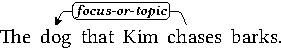
\includegraphics{pdf/the-dog-which-Kim-chases-barks-1.pdf}} \\
b. & \evnup{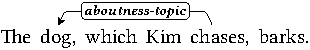
\includegraphics{pdf/the-dog-which-Kim-chases-barks-2.pdf}} \\
\end{tabular}}}



Because \tdl{aboutness-topic} is a subtype of \tdl{focus-or-topic} all
relative clauses can be understood as inheriting from rel-clause as
defined in \myref{avm:rel-clause}.\is{topic}


\myexe{\enumsentence{\label{avm:rel-clause}
\evnup{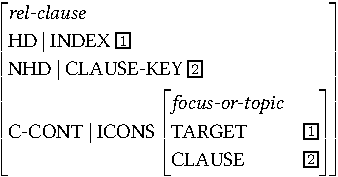
\includegraphics{pdf/rel-clause.pdf}}}}


\noindent Note that the information structure relation that the
relativized NPs have to the relative clauses should be
constructionally added using C-CONT, because the meaning is specified
at the phrasal level.  The phrase structure type responsible for
non-restrictive relative clauses requires us to impose a more specific
value (i.e.\ \tdl{aboutness-topic}). This is left to future work.



\largerpage[-1]
\section{Adverbial clauses}
\label{10:ssec:adjunct}

Adverbial clauses in the current analysis may be evaluated as having a
relation of either \tdl{topic} or just the underspecified value
\tdl{info-str} with respect to the main clauses.\is{underspecification}  The choice depends
on the type of subordinating conjunction and the details are
elaborated in the subsections below.\footnote{Using this strategy,
  subordinating conjunctions sometimes introduce an underspecified
  \tdl{info-str} element into \isi{ICONS} like verbal items that take
  clausal complements (Section \ref{10:ssec:embedded}).These underspecified
  elements are disadvantageous as mentioned in the first footnote of
  the current chapter, and a revised analysis in future work will
  suppress this problem.}


\subsection{Background} 
\label{10:ssec:adjunct:background}



Several previous studies investigate conditional \textit{if}-clauses
and temporal \textit{when}-clauses with respect to topichood.\is{topic}
\citet{haiman:78} argues that conditionals are topics, and
\citet{ramsay:87} also argues that \textit{if}/\textit{when} clauses
are endowed with topichood when they precede the main clauses.
Implicit in these claims is the argument that
\textit{if}/\textit{when} clauses differ in their information
structure depending on whether they are at the beginning, at the end,
and in the middle of an utterance.  Traditional movement-based studies
account for variation in conditional and temporal clauses in terms of
the so-called Adjunct Island Constraint \citep{huang:82}:
Postposed conditional and temporal clauses are adjoined to VPs forming
an adjunct island, while preposed ones are moved into IP's specifier
position \citep{iatridou:91} or generated in situ
\citep{taylor:07}.  In other words, preposed adverbial clauses modify
the main sentence, while postposed ones modify the VP.



Consequently, conditional and temporal clauses have a \isi{topic} feature
when they are sentence-initial.  Following this line of reasoning, the
present work assumes that topic is associated with preposed
conditional and temporal clauses with respect to the main
clauses. Syntactically, because they appear in the sen\-tence-initial
position and their function is to restrict the domain of what the
speaker is talking about, they are understood as \tdl{frame-setting}
as presented in
Figure~\ref{fig:sform} \mypage{fig:sform}.\is{sentential forms} With
respect to sentence-final/internal conditional and temporal clauses,
their information structure relation to the main clause parsimoniously
remains underspecified.\is{frame-setting}\is{underspecification}



\subsection{Analysis}
\label{10:ssec:adjunct:analysis}

Before analyzing adverbial clauses,\is{adverbial clause} it is
necessary to look at the information structure relationship between
adverbs and their clauses.\is{frame-setter} Frame-setters, as
discussed previously, have several restrictions: (i) they normally
appear initially, (ii) they can multiply occur in a single clause, and
(iii) they should play a role in restricting the domain of what the
speaker is talking about (e.g.\ spatial, temporal, manner, or
conditional).\is{clause-initial} First, the clause-initial constraint
can be conditioned by \mbox{[L-PERIPH +]}, which renders the
constituents left-peripheral.\is{periphery} The second constraint can
be enforced by \tdl{sform},\is{\textit{sform}} as presented in
Chapter~\ref{chapter9}, namely \tdl{frame-setting} \vs
\tdl{non-frame-setting}.\is{L-PERIPH} The third constraint is
potentially controversial, because information about lexical semantics
has not yet been included into the \isi{DELPH-IN} reference
formalism. Future work would then reference lexical semantic
information to identify whether a given adverb conveys a spatial,
temporal, or manner meaning.\footnote{There is some on-going research
  which seeks to incorporate lexical semantic information within
  \isi{DELPH-IN} grammars using WordNets
  \citep{bond:etal:09,pozen:13}.}




The combination of a \isi{frame-setting} adverb with the rest of
sentence should be carried out using a specific subtype of
\tdl{head-mod-phrase}, meaning that \tdl{head-mod-phrase} needs to be
divided into at least two subtypes; one requiring [L-PERIPH +] of its
NON-HEAD-DTR, and the other requiring [L-PERIPH --] of both
daughters.\is{L-PERIPH} The former imposes an \tdl{info-str}
constraint on the NON-HEAD-DTR. Thereby, the sentence-initial adverb
\textit{today} in \myref{fig:today:loudly} has a \tdl{topic} relation
to the main verb \textit{barks}.




\myexe{\enumsentence{\label{fig:today:loudly}
\evnup{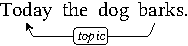
\includegraphics{pdf/today.pdf}}}}



\noindent Note that the mother node of \tdl{frame-setting} has an
underspecified value for L-PERIPH (i.e.\ [L-PERIPH
  \textit{luk}]). Thus, \textit{today the dog barks} with the
frame-setter \textit{today} can serve as the head-daughter of another
\tdl{frame-setting} construction, such as \textit{At home today the
  dog barks.} In this analysis, each frame-setter (e.g.\ \textit{at
  home} and \textit{today}) has its own \tdl{topic} relation to the
verb.\is{topic}


In \ili{Japanese} and \ili{Korean}, \wa and \nun can be attached to
adjuncts. If they are adjacent to adjuncts, the constituents are
normally evaluated as bearing \isi{contrastiveness}. If an adjunct is
combined with \wa or \nun, the adjunct should be associated with
\tdl{contrast},\is{contrast} even when it appears in the leftmost
position. Consequently, \textit{kyoo} `today' in the left-peripheral
position has a plain \tdl{topic} relation, while \textit{kyoo-wa}
`today-wa' has a \tdl{contrast-topic} relation to the verb
\textit{hoeru} `bark'.\is{periphery}\is{topic}


\myexe{\enumsentence{\toplabel{exe:kyoo}
\shortex{5}
{kyoo & (wa) & inu & ga & hoeru.}
{today & (\textsc{wa}) & dog & \textsc{nom} & bark}
{`Today, the dog barks.' [jpn]}}}

\myexe{\enumsentence{\label{fig:kyoo}
\begin{tabular}[t]{lllll}
a. & \evnup{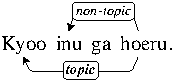
\includegraphics{pdf/kyoo.pdf}} & & b. &
\evnup{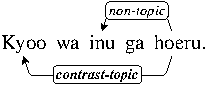
\includegraphics{pdf/kyoo-wa.pdf}} \\
\end{tabular}}}




Regarding adverbial clauses,\is{adverbial clause} my argument is that
subordinating conjunctions are responsible for the information
structure relation between adverbial clauses and main
clauses.\is{adverbial clause} First of all, subordinating conjunctions
that entail temporal and conditional clauses signal \tdl{topic}
\citep{haiman:78,ramsay:87}, as discussed above. Other subordinating
conjunctions assign an underspecified \tdl{info-str} value, because
there seems to be no clear distinction of information structure
status. Causal conjunctions, such as \textit{because} in \ili{English} and
\textit{weil} in German, do not show consistency in information
structure \citep{heycock:07}, which means there is no lexical and
phrasal clue to identify the information structure
relations.\footnote{The meaning could be clear by a specific prosodic
  pattern, like intonation.}  It is even less clear how concessive
conjunctions, such as (\textit{al})\textit{though}, configure
information structure, though they are known to be partially related
to information structure \citep{chung:kim:09}.\is{underspecification}
They are also provisionally treated as underspecified in this analysis. Some
conjunctions with multiple meanings, such as \textit{as}, are also
assumed to assign an underspecified value, because we cannot 
clearly identify the associated information structure meanings in the
absence of contextual information.\is{ICONS-KEY}




\myexe{\enumsentence{\label{avm:when}
\evnup{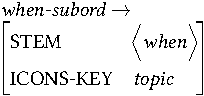
\includegraphics{pdf/when-lex.pdf}}}}


All subordinate conjunctions have one \tdl{info-str} value on their
ICONS list. However, they do not inherit from any \tdl{icons-lex-item}
presented in Chapter~\ref{chapter9}.\is{CLAUSE}\is{TARGET} This is
because in this case TARGET should point to the semantic head (usually
a verb) of the adverbial clause, rather than the conjunction itself,
and also because the CLAUSE is readily and lexically identified to be
the INDEX of the main clause.  The following AVM presents this
co-indexation.


\myexe{\enumsentence{\label{avm:subconj-word}
\evnup{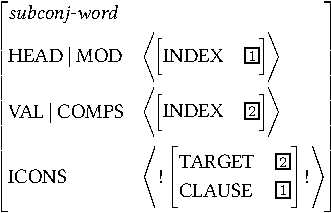
\includegraphics{pdf/subconj-word.pdf}}}}


\noindent As a consequence, adverbial clauses have the information
structure relation to the main clauses exemplified in
\myref{fig:when:because}. The arrows from \textit{reads} to
\textit{barks} at the bottom are created by \myref{avm:subconj-word}.
The value \tdl{topic} on the arrow of (\ref{fig:when:because}a) is
specified in \myref{avm:when}.\is{topic} In addition, the arrow of
(\ref{fig:when:because}b) is specified as merely \tdl{info-str}, since
the subordinate conjunction is devoid of any similar constraint.




\myexe{\eenumsentence{\toplabel{fig:when:because}
\item\evnup{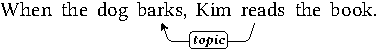
\includegraphics{pdf/when.pdf}}
\item\evnup{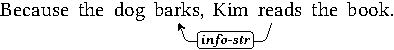
\includegraphics{pdf/because.pdf}}}}



\section{Summary}
\label{10-2:ssec:Summary}


This chapter has addressed how information structure in multiclausal
utterances is represented via \isi{ICONS} and what kinds of
constraints are imposed on non-matrix clauses.\is{complement clause}
There are three types of non-matrix clauses that this chapter
explores: complement clauses, relative clauses, and adverbial
clauses.\is{complement clause}\is{relative clause}\is{adverbial
  clause} First, the information structure relation between matrix
clauses and their complement clauses largely depends on the verbal
type of the main predicate. In particular, if the predicate serves to
invoke an assertion regarding the complement clause, the complement
clause has a \tdl{focus} relation to the main clause.\is{relative
  clause}\is{focus} Second, information structure relations between head nouns
and associated relative clauses depend on the reading of the
particular relative clauses. If the relative is restrictive, the head
nouns are assigned a \tdl{focus-or-topic} interpretation by the
relative clauses. Otherwise, they are assigned the more specific type
\tdl{aboutness-topic}.\is{aboutness topic} Third, information structure in adverbial
clauses is influenced by the position of the clauses and the type
of conjunction. If the adverbial clause is temporal or conditional and
appears sentence-initially, it is assigned a \tdl{topic}
interpretation. Other adverbial clauses are preferentially
underspecified.\is{underspecification}



